\section{Unsupervised learning}

\begin{frame}{Unsupervised learning: Motivation}
    \begin{tikzpicture}
        \node[] at (-5.25, 3.5) {};
        \node[] at (-5.25, -3.5) {};

        \node[anchor=north west, font=\bfseries] at (-5, 3) {
            \underline{Supervised learning}: Find $\mathbf{\hat{y}=f(X)}$
        };
        \visible<2-8>{
            \node[anchor=north west, text width=10.5cm, align=left] at (-5, 2.7) {
                \begin{itemize}
                    \item Descriptive: Understand the relationship between $X$ and $y$
                    \item <3-> Predictive: Predict $y$ given new $X$.
                    \begin{itemize}
                        \item <4-> Because the predictions are useful
                        \item <5-> Because we want to know if it is possible
                    \end{itemize}
                \end{itemize}
            };
        }
        \visible<2>{
            \node[] at (0, -1) {
                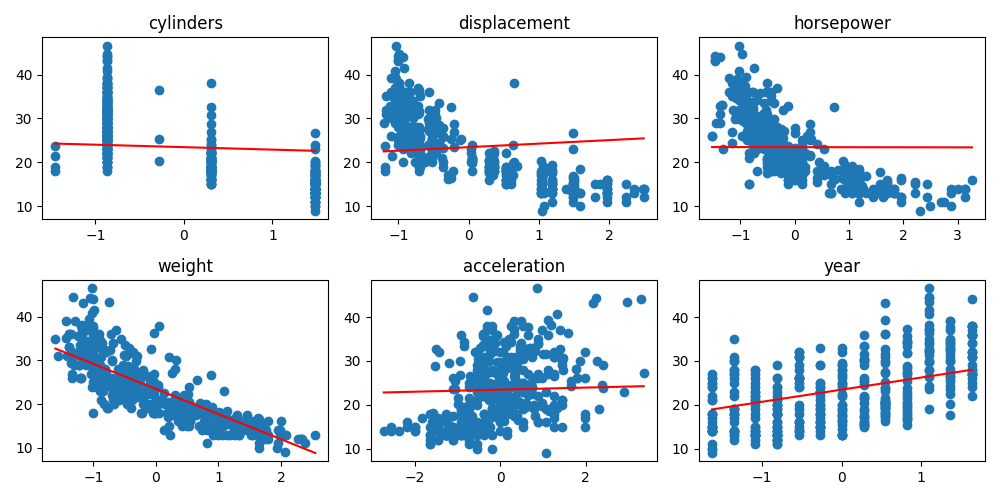
\includegraphics[height=4cm]{data/coefficients.png}
            };
        }
        \visible<4>{
            \node[] at (0, -1.5) {
                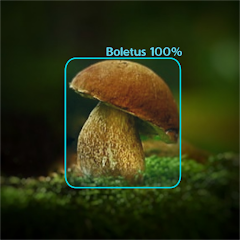
\includegraphics[height=3cm]{data/mushroom.png}
            };
        }
        \visible<5>{
            \node[] (mri) at (-2, -1.5) {
                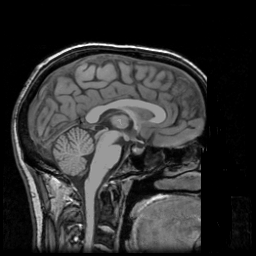
\includegraphics[height=2.5cm]{data/brain.png}
            };
            \node[draw=black, dashed] (outcome) at (2, -1.5) {
                Depression?
            };
            \draw[-stealth, line width=5pt, gray] (mri) -- (outcome);
        }
        \visible<6-8>{
            \node[anchor=north west, font=\bfseries] at (-5, 0) {
                \underline{Unsupervised learning}: Are there interesting patterns in $\mathbf{X}$?
            };
        }
        \visible<7-8>{
            \node[anchor=north west, text width=10.5cm, align=left] at (-5, -0.3) {
                \begin{itemize}
                    \item Can we find subgroups or interesting axes of variability?
                    \item <8> Exploratory analyses
                    \item <8> Visualization
                \end{itemize}
            };
        }
    \end{tikzpicture}
\end{frame}
